\documentclass{article}
\usepackage{amsmath, tikz, enumerate, sfmath, multicol, tcolorbox}
\renewcommand{\familydefault}{\sfdefault}
\usepackage[top = 0.5in, bottom = 0.5in, left = 1in, right = 1in]{geometry}
\pagestyle{empty}
\raggedright
\tikzset{>=stealth}

\newcounter{example}[section]
\newenvironment{example}[1][]{\refstepcounter{example}\par\medskip
   {\color{red}\textbf{Example~\theexample. #1}}}{\medskip}
\begin{document}


\section*{Matrices}

\begin{tcolorbox}[colframe=orange!70!white, coltitle=black, title=\textbf{Summary}]
\begin{enumerate}
    \item Matrices are 2 or more vectors in the coordinate plane.
\end{enumerate}
\end{tcolorbox}
\bigskip 

A \textbf{matrix} is a rectangular array of numbers. It can be composed of vectors (or possibly scalars).	
\bigskip 

When listing the dimensions of a matrix, we note the number of rows, followed by the number of columns. 
\bigskip 

Matrix $A$ below has 3 rows and 4 columns, and has dimensions 3 by 4.
\bigskip 
\[	A = \begin{bmatrix}
8 & 6 & 7 & 5 \\
3 & 0 & 9 & -2 \\
0 & 1 & -10 & 7 
\end{bmatrix}
\]
\bigskip 


Each of the values in a matrix are called \textbf{elements}. In matrix $A$, the element in the 1st row, 2nd column is 6 and is denoted
\[ a_{12} = 6 \]
\bigskip 

We can think of a matrix as several vectors in the coordinate plane. \newline 

\begin{minipage}{0.3\textwidth}
\[
\begin{bmatrix}
{\color{blue}\pmb{3}} & {\color{red}\pmb{-1}} & {\color{violet}\pmb{-5}} \\
{\color{blue}\pmb{2}} & {\color{red}\pmb{-4}} & {\color{violet}\pmb{3}} 
\end{bmatrix}
\]
\end{minipage}
\begin{minipage}{0.6\textwidth}
    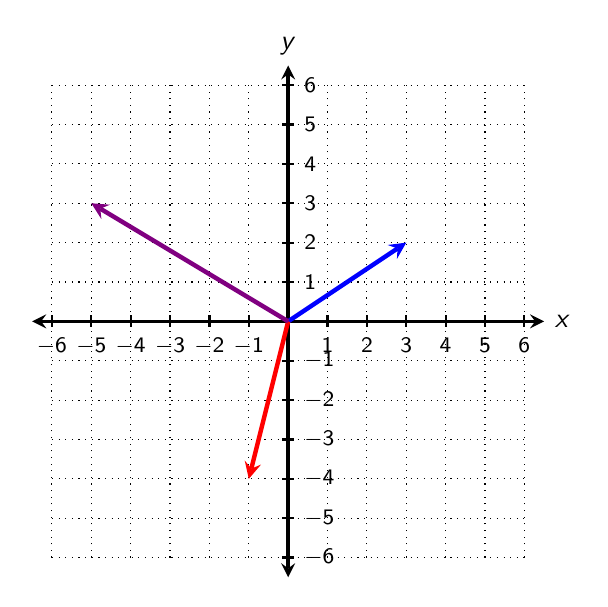
\begin{tikzpicture}[scale=0.5]
    \draw[dotted] (-6,-6) grid (6,6);
    \draw[<->, very thick] (-6.5,0) -- (6.5,0) node [right] {$x$};
    \draw[<->, very thick] (0,-6.5) -- (0,6.5) node [above] {$y$};
    \foreach \x in {-6,...,-1,1,2,...,6}
    \draw [thick] (\x, 0.15) -- (\x, -0.15) node [below] {\footnotesize $\x$};
    \foreach \y in {-6,...,-1,1,2,...,6}
    \draw [thick] (-0.15, \y) -- (0.15, \y) node [right] {\footnotesize $\y$};
    \draw[->, ultra thick, blue] (0,0) -- (3,2);
    \draw[->, ultra thick, red] (0,0) -- (-1,-4);
    \draw[->, ultra thick, violet] (0,0) -- (-5,3);
    \end{tikzpicture}
\end{minipage}
\bigskip 

\begin{example}
Graph the matrix $\begin{bmatrix}
1 & 0 \\
0 & 1
\end{bmatrix}$
\bigskip 
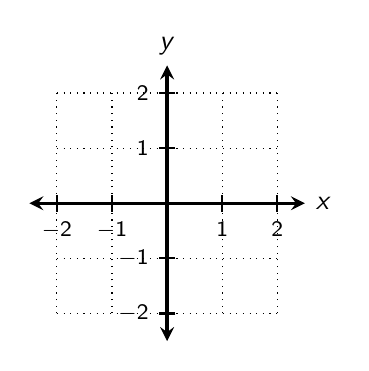
\begin{tikzpicture}[scale=0.7]
\draw[dotted] (-2,-2) grid (2,2);
\draw[<->, very thick] (-2.5,0) -- (2.5,0) node [right] {$x$};
\draw[<->, very thick] (0,-2.5) -- (0,2.5) node [above] {$y$};
\foreach \x in {-2,-1,1,2}
\draw [thick] (\x, 0.15) -- (\x, -0.15) node [below] {\footnotesize $\x$};
\foreach \y in {-2,-1,1,2}
\draw [thick] (0.15, \y) -- (-0.15, \y) node [left] {\footnotesize $\y$};
\end{tikzpicture}
\end{example}
\newpage

\subsection*{Matrix Addition and Subtraction}

If two matrices have the same dimensions, then we can add and subtract them. \newline\\

To do this, we add (or subtract) corresponding elements just like vector addition and subtraction.	\newline\\

\begin{example}
Given matrices 
\[
A = \begin{bmatrix}
-2 & 3 \\
0 & 4 
\end{bmatrix}
\quad
B = \begin{bmatrix}
4 & -3 \\
-2 & -1
\end{bmatrix}
\quad
C = \begin{bmatrix}
-7 & 6 & -1 \\
0 & 4 & -4 
\end{bmatrix}
\]
find each and graph your answers (if possible).  \newline

\begin{enumerate}[(a)]
\begin{multicols}{2}
    \item $A + B$
    \item $B + A$
\end{multicols}
\end{enumerate}
\begin{minipage}{0.5\textwidth}
    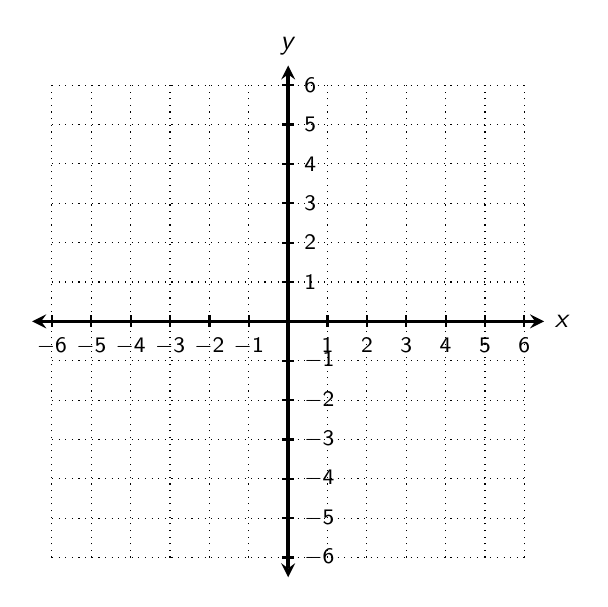
\begin{tikzpicture}[scale=0.5]
    \draw[dotted] (-6,-6) grid (6,6);
    \draw[<->, very thick] (-6.5,0) -- (6.5,0) node [right] {$x$};
    \draw[<->, very thick] (0,-6.5) -- (0,6.5) node [above] {$y$};
    \foreach \x in {-6,...,-1,1,2,...,6}
    \draw [thick] (\x, 0.15) -- (\x, -0.15) node [below] {\footnotesize $\x$};
    \foreach \y in {-6,...,-1,1,2,...,6}
    \draw [thick] (-0.15, \y) -- (0.15, \y) node [right] {\footnotesize $\y$};
    \end{tikzpicture}
\end{minipage}
\begin{minipage}{0.45\textwidth}
    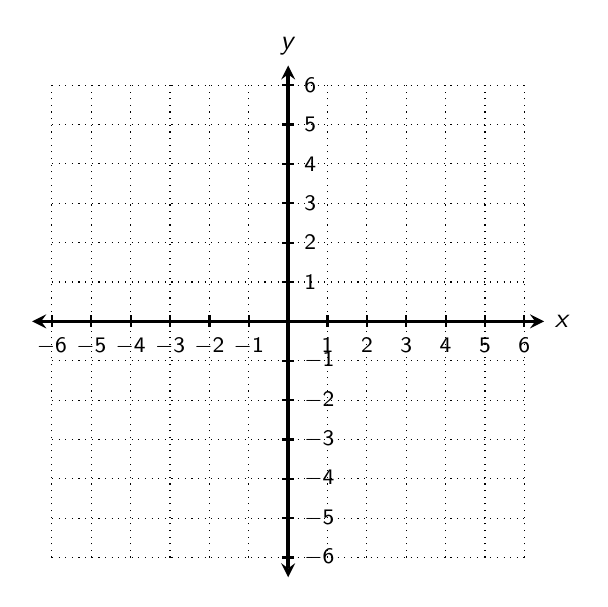
\begin{tikzpicture}[scale=0.5]
    \draw[dotted] (-6,-6) grid (6,6);
    \draw[<->, very thick] (-6.5,0) -- (6.5,0) node [right] {$x$};
    \draw[<->, very thick] (0,-6.5) -- (0,6.5) node [above] {$y$};
    \foreach \x in {-6,...,-1,1,2,...,6}
    \draw [thick] (\x, 0.15) -- (\x, -0.15) node [below] {\footnotesize $\x$};
    \foreach \y in {-6,...,-1,1,2,...,6}
    \draw [thick] (-0.15, \y) -- (0.15, \y) node [right] {\footnotesize $\y$};
    \end{tikzpicture}
\end{minipage}
\vfill 

\begin{enumerate}[(a)]  \setcounter{enumi}{2}
\begin{multicols}{2}
    \item $A - B$
    \item $A + C$
\end{multicols}
\end{enumerate}
\begin{minipage}{0.5\textwidth}
    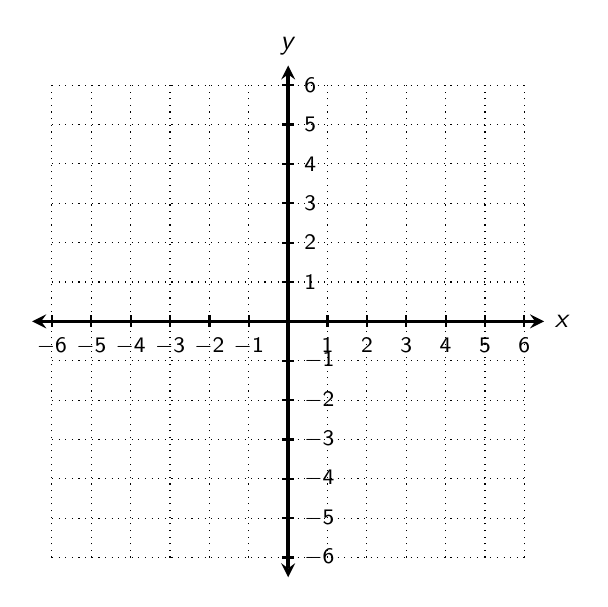
\begin{tikzpicture}[scale=0.5]
    \draw[dotted] (-6,-6) grid (6,6);
    \draw[<->, very thick] (-6.5,0) -- (6.5,0) node [right] {$x$};
    \draw[<->, very thick] (0,-6.5) -- (0,6.5) node [above] {$y$};
    \foreach \x in {-6,...,-1,1,2,...,6}
    \draw [thick] (\x, 0.15) -- (\x, -0.15) node [below] {\footnotesize $\x$};
    \foreach \y in {-6,...,-1,1,2,...,6}
    \draw [thick] (-0.15, \y) -- (0.15, \y) node [right] {\footnotesize $\y$};
    \end{tikzpicture}
\end{minipage}
\begin{minipage}{0.45\textwidth}
    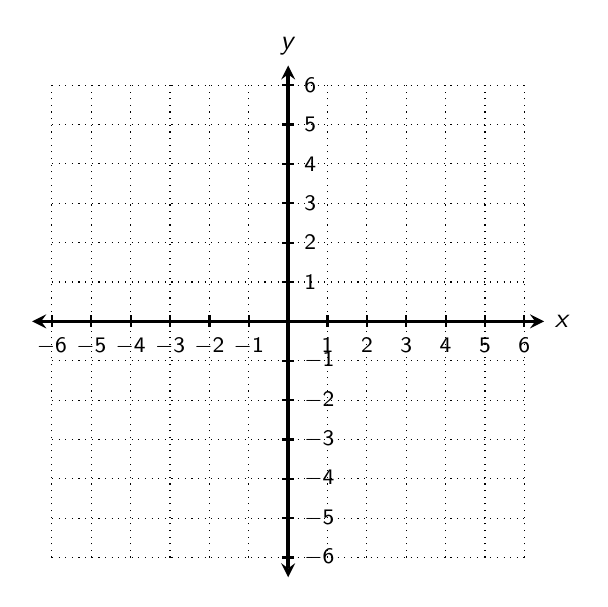
\begin{tikzpicture}[scale=0.5]
    \draw[dotted] (-6,-6) grid (6,6);
    \draw[<->, very thick] (-6.5,0) -- (6.5,0) node [right] {$x$};
    \draw[<->, very thick] (0,-6.5) -- (0,6.5) node [above] {$y$};
    \foreach \x in {-6,...,-1,1,2,...,6}
    \draw [thick] (\x, 0.15) -- (\x, -0.15) node [below] {\footnotesize $\x$};
    \foreach \y in {-6,...,-1,1,2,...,6}
    \draw [thick] (-0.15, \y) -- (0.15, \y) node [right] {\footnotesize $\y$};
    \end{tikzpicture}
\end{minipage}
\end{example}

\vfill 
\newpage 


\subsection*{Scalar Multiplication}

We saw how scalars affect vectors. \newline\\

Since a matrix can be thought of as an array of vectors,

multiplying a matrix by a scalar has the same effect that multiplying a vector by a scalar does:  

\begin{center}
\textbf{Each element in the matrix gets multiplied by the scalar.}\end{center}

\begin{example}
Using \[
A = \begin{bmatrix}
-2 & 3 \\
0 & 5 
\end{bmatrix}
\quad
B = \begin{bmatrix}
4 & -3 \\
-2 & -1
\end{bmatrix}
\quad
C = \begin{bmatrix}
-7 & 6 & -1 \\
0 & 4 & -4 
\end{bmatrix}
\]
find each.  \newline\\

\begin{enumerate}[(a)]
\begin{multicols}{3}
    \item $5A$
    \item $-1C$
    \item $5A + 2B$
\end{multicols}
\end{enumerate}
\end{example}



\end{document}
